
\section{Equations of Motion \& Free Body Diagrams}

Equations of Motions (EOM) and free body diagrams (FBD) are the cornerstones of any dynamics. 
Determining how the vectors and forces are applied to the different bodies, a calculation of moment and force of each body can be managed.\\
In figure \ref{fig:FBD} torques, lengths, different forces and vectors are Illustrated. By equating these, as seen in table \ref{tab:EoM}, force and motion for each body is determined.\\
These equations can then be used with the kinematics of the CrustCrawler, to determine position-vectors, torques and velocity-vectors.

\begin{figure}[H]
    \centering
    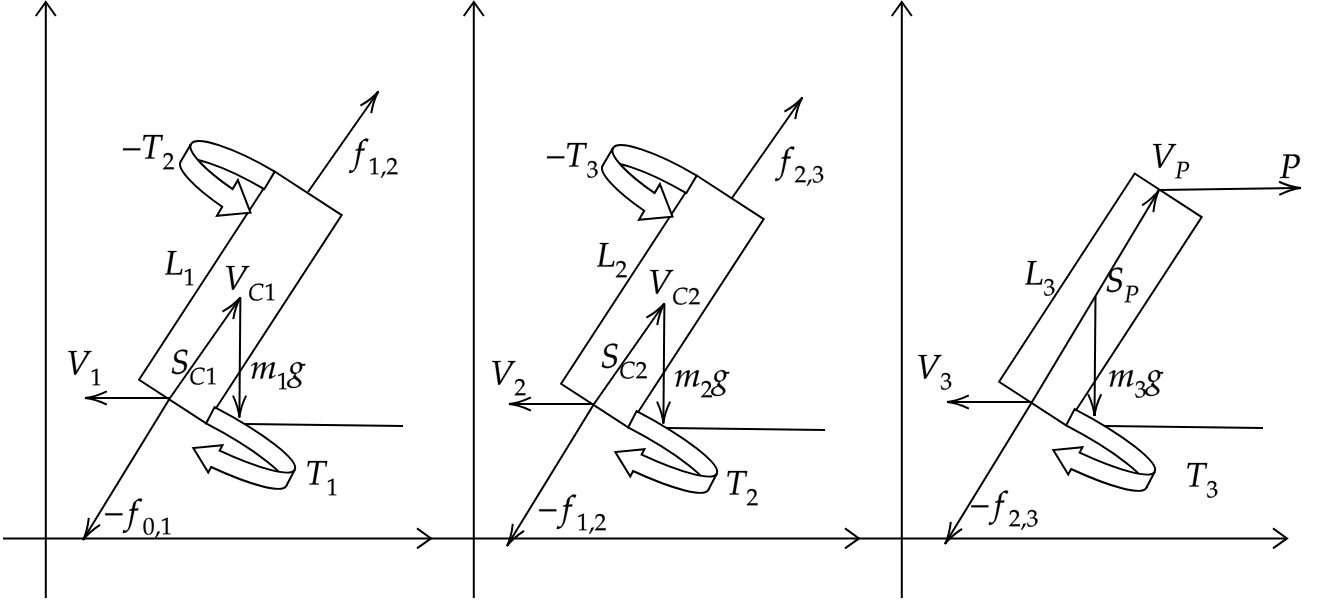
\includegraphics[width=14cm,height=5cm]{Figures/Technical_figures/FBD.png}
    \caption{Free body diagrams(FBD). All torques, lengths, different forces and vectors can be seen, by Equating these every force and motion of each body can be calculated}
    \label{fig:FBD}
\end{figure}

\begin{table}[H]
  \centering
\begin{tabular}{ |P{1.5cm}||P{4cm}||P{5cm}|}
 \hline
 \multicolumn{3}{|c|}{\textbf{Equations of Motion}} \\
 \hline
 Body & \(\sum F=ma\) & \(\sum M=I\alpha\)  \\
 \hline
 1 & \(-f_0_,_1+f_1_,_2+m_1g\) & \(\tau_1-\tau_2+(-S_C_1)\underline{X}(-f_0_,_1)+(S_1-S_C_1\underline{X}(f_1_,_2)\)  \\[7pt]
 \hline
 2 & \(-f_1_,_2+f_2_,_3+m_2g\) & \(\tau_2-\tau_3+(-S_C_2)\underline{X}(-f_1_,_2)+(S_2-S_C_2)\underline{X}(f_2_,_3)\) \\[7pt]
 \hline
 3 & \(-f_2_,_3+P\) & \(\tau_3+(-S_P)\underline{X}(-f_2_,_3)\) \\[7pt]
\hline
 \end{tabular}
 \caption{Equations of Motions for each body}
    \label{tab:EoM}
\end{table}

\section{Recursive Newton-Euler}
The first approach which has been made to determine the dynamics of the CrustCrawler bodies is the recursive Newton-Euler method through an inwards and outwards calculation. \\
Outward dynamics is the calculation of acceleration of each body from base to end-effector.\\
Inward dynamics is the calculation of forces on each body from end-effector to base.\\

\iffalse
\begin{table}[H]
  \centering
\begin{tabular}{|P{2cm}||P{4cm}||P{4cm}|}
 \hline
 \multicolumn{3}{|c|}{\textbf{Preconditions of Recursive method}} \\[7pt]
 \hline
& Angle     &   Angular velocity\\
Length & \(\theta\) & \(\omega\) \\
 \hline
  \hline
  & & \\
 L1 = 70 & \(\theta_1=\dfrac{\pi}{6}\) & \(\omega_1=\dfrac{\pi}{4}\) \\[1pt]
 & & \\
 \hline 
 & & \\
 L2 = 210 &\(\theta_2=\dfrac{\pi}{6}\) &\(\omega_2=\dfrac{5\pi}{12}\) \\[1pt]
 & & \\
 \hline
 & & \\
 L3 = 219 &\(\theta_3=\dfrac{-\pi}{3}\) &\(\omega_3=\dfrac{\pi}{12}\) \\[1pt]
& & \\
\hline
 \end{tabular}
 \label{EoM}
\end{table}
\fi

\begin{table}[H]
  \centering
\begin{tabular}{|P{4cm}||P{4cm}||P{4cm}|}
 \hline
 \multicolumn{3}{|c|}{\textbf{Preconditions of Recursive method}} \\[7pt]
 \hline
 Angle     &   Angular velocity  &  Reference velocity\\
 \(\theta\) & \(\omega\) & \(\dot\theta\)\\
 \hline
  \hline
  && \\
  \(\theta_1=\dfrac{\pi}{6}\) & \(\omega_1=\dfrac{\pi}{4}\) & \(\dot\theta_3=\dfrac{\pi}{4} \) \\[1pt]
  &&\\
 \hline 
  && \\
\(\theta_2=\dfrac{\pi}{6}\) &\(\omega_2=\dfrac{5\pi}{12}\) & \(\dot\theta_3=\dfrac{\pi}{6}\) \\[1pt]
  && \\
 \hline
  & &\\
 \(\theta_3=\dfrac{-\pi}{3}\) &\(\omega_3=\dfrac{\pi}{12}\) & \(\dot\theta_3=\dfrac{-\pi}{3}\) \\[1pt]
 & &\\
\hline
 \end{tabular}
 \caption{Preconditions of Recursive method} 
 \label{EoM}
\end{table}%\

\noindent
The first step is to find the position-vectors of the bodies introduced in figure \ref{fig:FBD}.\\
This step is crucial for the recursive method, since the forces of the bodies will be added onto these vectors. To elaborate, it is known that forces on a larger object will create more torque and more acceleration needed than on a smaller object. Hereby the preconditions is of most importance to get the correct acceleration or force. \\
To find the vectors a simple mathematical approach is used:\\
finding the vectors at the Center of Mass(C.O.M) can be done by taking the length of the body and adding the different thetas in the x and y-axis direction. The vector which runs through the whole body can be found using the same approach, but utilising the whole length of the body.\\

 \begin{align}
     S_C_1&&=&&
\left[\begin{matrix}
    \dfrac{L_1}{2}\cdot \cos{\theta_1} \\[6pt]
    \dfrac{L_1}{2}\cdot \sin{\theta_1}
\end{matrix}\right]&&\Rightarrow&&
\left[\begin{matrix}
    30.312 \\[6pt]
    17.5
\end{matrix}\right]\\\notag 
\\
    S_1 &&=&&
\left[\begin{matrix}
    L_1\cdot \cos{\theta_1} \\[6pt]
    L_1\cdot \sin{\theta_1}
\end{matrix}\right]&&\Rightarrow&& 
\left[\begin{matrix}
    60.62 \\[6pt]
    35
\end{matrix}\right]\\\notag
\end{align}
\begin{align}
    \phi_1 &&=&& \theta_1+\theta_2 &&=&& \dfrac{\pi}{3}
\end{align}
\\

\begin{align} 
   S_C_2 &&=&&
\left[\begin{matrix}
    \dfrac{L_2}{2}\cdot \cos{\phi_1} \\[6pt]
    \dfrac{L_2}{2}\cdot \sin{\phi_1}
\end{matrix}\right]&&\Rightarrow&&
\left[\begin{matrix}
    52.50 \\[6pt]
    90.93
\end{matrix}\right]\\\notag
\\
    S_2 &&=&&
\left[\begin{matrix}
    L_2\cdot \cos{\phi_1\degree} \\[6pt]
    L_2\cdot \sin{\phi_1\degree}
\end{matrix}\right]&&\Rightarrow&&
\left[\begin{matrix}
    105 \\[6pt]
    181.87
\end{matrix}\right]\\\notag
\end{align}
\begin{align}
    \phi_2&&=&&\phi_1+\theta_3&&=&&0
\end{align}
\\
\begin{align}
    S_C_P &&=&&
\left[\begin{matrix}
    \dfrac{L_3}{2}\cdot \cos{\phi_2} \\[6pt]
    \dfrac{L_3}{2}\cdot \sin{\phi_2}
\end{matrix}\right]&&\Rightarrow&&
\left[\begin{matrix}
    109.5 \\[6pt]
    0
\end{matrix}\right]\\\notag
\\
    S_P &&=&&
\left[\begin{matrix}
    L_3\cdot \cos{\phi_2} \\
    L_3\cdot \sin{\phi_2}
\end{matrix}\right]&&\Rightarrow&&
\left[\begin{matrix}
    219 \\
    0
\end{matrix}\right]
\end{align}


The different velocities for each body can now be found, by using the outward recursive formulas:\\
As seen below there is three different points which the velocity takes place around. The first is the angular velocity, which is given by:\\
\begin{equation}\label{eq:W}
\omega_i=\omega_i-_1+\dot\theta_i
\end{equation}\\
The second, \(V_i\), is calculating the velocity around the hinges, which is also known as the inertia tensors, are given by:\\
\begin{equation}\label{eq:Vi}
V_i=V_i_-_1+\omega_i_-_1\cdot Z\underline{X}S_i
\end{equation}\\
 \(V_C_i\) is the point in the Center Of Mass (C.O.M) of the body. By calculating the velocity around the point the angular velocity of the C.O.M can be found. The mathematically approach of this calculation is given by:\\
\begin{equation}\label{eq:Vci}
V_C_i=V_i-_1+\omega_i-_1\cdot Z\underline{X}S_C_i
\end{equation}

\begin{align}
    V_1&&=&& &&=&&
\left[\begin{matrix}
    0\\
    0\\
    0
\end{matrix}\right]\\ V_C_1&&=&&V_1+\omega_1\cdot Z\underline{X}S_C_1&&=&&\left[\begin{matrix}
    -4.37\pi\\
    7.57\pi\\
    0
\end{matrix}\right]\\
    V_2&&=&&0+\omega_1\cdot Z\underline{X}S_1&&=&&
\left[\begin{matrix}
    -14.58\pi\\
    25.25\pi\\
    0
\end{matrix}\right]\\ V_C_2&&=&&V_2+\omega_2\cdot Z\underline{X}S_C_2&&=&&
\left[\begin{matrix}
   -45.80-37.88\pi \\
    79.32+21.87\pi\\
    0
\end{matrix}\right]\\
    V_3&&=&&V_2+\omega_2\cdot Z\underline{X}S_2&&=&&
\left[\begin{matrix}
    -45.80-15.15\pi\\
    79.32+8.70\pi\\
    0
\end{matrix}\right]\\ V_P&&=&&V_3&&=&&\left[\begin{matrix}
    45.80-15.15\pi\\
    79.32+8.70\pi\\
    0
\end{matrix}\right]
\end{align}
\\
Now that the velocities are known the accelerations at the same points can be found.\\
By proceeding to the acceleration, some alteration has to be taken into consideration. For example, the product of velocity on each point of interest, e.g, equations \ref{eq:Vi} and \ref{eq:Vci}, will now be used as a reference point to get the accelerations as seen in equation \ref{eq:dotV} and \ref{eq:dotVc} :

\begin{equation}\label{eq:dotomega}
\dot\omega_i=\dot\omega_i-_1+\ddot\theta_i
\end{equation}

\begin{equation}\label{eq:dotV}
\dot{V}_i=\dot{V}_i_-_1+\dot\omega_i_-_1\cdot Z\underline{X}S_i_-_1+\omega_i_-_1\cdot Z\underline{X}(\omega_i_-_1\cdot\underline{X}S_i_-_1)
\end{equation}

\begin{equation}\label{eq:dotVc}
\dot{V}_C_i=\dot{V}_i+\dot\omega_i\cdot Z\underline{X}S_C_i+\omega_i\cdot Z\underline{X}(\omega_i\cdot\underline{X}S_C_i)
\end{equation}
\\
In the next equations the result will be represented, not the calculation, since the course of action can be seen above in equation \ref{eq:dotomega}, \ref{eq:dotV} and \ref{eq:dotVc}.\\

\begin{align}
\dot\omega_1=\dfrac{\pi}{6}&&
    \dot{V}_1&&=
\left[\begin{matrix}
    0\\
    0\\
    0
\end{matrix}\right]&&,&&\dot{V}_C_1&&=\left[\begin{matrix}
    -27.40\\
    5.22\\
    0.
\end{matrix}\right]\\
\dot\omega_2=\dfrac{\pi}{12}&&
    \dot{V}_2&&=
\left[\begin{matrix}
    -55.33\\
    9.86\\
    0.
\end{matrix}\right]&&,&& \dot{V}_C_2&&=
\left[\begin{matrix}
   -167.99 \\
   -130.77\\
    0
\end{matrix}\right]\\
\dot\omega_3=\dfrac{\pi}{3}&&
    \Dot{V}_3&&=
\left[\begin{matrix}
    -282.37\\
    -271.72\\
    0
\end{matrix}\right]&&,&& \dot{V}_P&&=\left[\begin{matrix}
    -282.37\\
    -271.72\\
    0
\end{matrix}\right]
\end{align}
\\
\noindent
Finally the accelerations of the system can be used with the inward calculations and equations. However before any calculations can be equated $f_c_i$ and $M_c_i$, has to be determined:\\
\begin{equation}\label{eq:fci}
    f_c_i=m_i\cdot \Dot{v}_i
\end{equation} 
\begin{equation}\label{eq:Mi}
    M_c_i=I_i\cdot \Dot{\omega}_i
\end{equation}


\begin{align}
    f_c_1=135\cdot \dot{v}_c_1=\left[\begin{matrix}
    -1.843\\
    3.210\\
    0
\end{matrix}\right]&&
    M_c_1=V_1\cdot \dot{\omega}_1=\left[\begin{matrix}
    0\\
    0\\
    0
\end{matrix}\right]\\
    f_c_2=36.8\cdot \dot{v}_c_2= \left[\begin{matrix}
    -5.9630\\
    0.3906\\
    0
\end{matrix}\right]&&
  M_c_2=V_2\cdot \dot{\omega}_2= \left[\begin{matrix}
    -11.9916\\
    20.7673\\
    0
\end{matrix}\right]\\
 f_c_3=22.7\cdot \dot{v}_c_3=\left[\begin{matrix}
    -0.0407\\
    1.1801\\
    0
\end{matrix}\right]&&
    M_c_3=V_3\cdot \dot{\omega}_3=\left[\begin{matrix}
    -97.8032\\
    111.6856\\
    0
\end{matrix}\right]
\end{align}

\noindent
Equation \ref{eq:fi} measures the applied forces of both inertial ,\(f_c_i\) seen in \ref{eq:fci}, and reaction forces \(f_i_,_i_+_1\). The equation is hereby given by:\\
\begin{equation}\label{eq:fi}
    f_i_-_1_,_i=f_c_i+f_i_,_i_+_1
\end{equation} \\

Equation \ref{eq:Mi}, calculates the whole system of each body with angular accelerations and applied forces. This equation is given by:\\

\begin{equation}\label{eq:Mi}
    M_i=M_c_i+m_i_+_1+S_c_i\underline{X}f_c_i+S_i\underline{X}f_i_,_i_+_i
\end{equation} \\

\noindent
Utilising equation \ref{eq:fi} and \ref{eq:fi}, forces applied to the body at two hinge points can be found.\\
\textbf{NB}, the equations below have a constant multiplier on each matrix which is $1.0e+0.3$, it is not computed into the matrix since it would apply a much larger result.

\begin{align}
    f_0_,_1=
\left[\begin{matrix}
    -1.8992\\
    3.2899\\
    0
\end{matrix}\right]&&
M_1=\left[\begin{matrix}
    0.0004\\
    0.0004\\
    3.9172
\end{matrix}\right]\\
    f_1_,_2=
\left[\begin{matrix}
    -6.0564\\
    0.4972\\
    0
\end{matrix}\right]&& 
M_2=
\left[\begin{matrix}
    0.0000\\
    0.0001\\
    1.7054
\end{matrix}\right]\\
    f_2_,_3=
\left[\begin{matrix}
    -0.1341\\
    1.2868\\
    0
\end{matrix}\right]&&
M_3=\left[\begin{matrix}
    -0.0006\\
    0.0015\\
    4.1048
\end{matrix}\right]
\end{align}
\\

\section{Lagrangian}
The Lagrangian is defined as the difference between the potential energy for a given system and the kinetic energy of the same system. The kinetic energy T, which is the work the body needs to accelerate and measured as the velocity combined with angular velocity;
\begin{equation}
   T=\dfrac{1}{2}\cdot m \cdot V^2 + \dfrac{1}{2}I\cdot \omega^2
\end{equation}
While V, the potential energy, can measure the gravity potential
\begin{equation}
  V=M_g\cdot h  
\end{equation}
and the elastic potential 
\begin{equation}
   V=\dfrac{1}{2}\cdot x^2 
\end{equation}
By substracting the kinetic and the potential energy, the langranian can be found.

\begin{equation}
    \mathcal{L}=T-V
\end{equation}

\subsection*{Lagrange equation}
The Lagrange equation states the following: The time derivative of the partial derivative Lagrangian with respect to the $\Dot{q}_i$ (generalised velocity) subtracted by the partial derivative Lagrangian with respect to the $q_i$ (generalised force) equals:
\begin{equation}
    Q_i = \frac{d}{dt}(\frac{\partial\mathcal{L}}{\parital \Dot{q_i}})-\frac{\partial\mathcal{L}}{\parital q_i}
\end{equation}
$Q_i$ is the generalised force for one body. The \textit{i} is referring to the D.O.F of the system, meaning that in the case of the CrustCrawler, there is the need to compute this 3 times with respect to the 3 D.O.F. as stated below by the known thetas:\\

\begin{align}
    Torque\ 1\ (\tau_1):&& \dfrac{d}{dt}\cdot\dfrac{\delta L_3}{\delta\dot{\theta_1}}-\dfrac{\delta L_3}{\delta\theta_1}&&=&&-4.8667Nm\\
    Torque\ 2\ (\tau_2):&& \dfrac{d}{dt}\cdot\dfrac{\delta L_3}{\delta \dot{\theta_2}}-\dfrac{\delta L_3}{\delta\theta_2}&&=&& 1.757Nm\\
    torque\ 3\ (\tau_3):&&\dfrac{d}{dt}\cdot\dfrac{\delta L_3}{\delta \dot{\theta_3}}-\dfrac{\delta L_3}{\delta\theta_3}&&=&&-1.663Nm
\end{align}
\\

By the known theory, Lagranian law,that states: \(q=\theta, and  \theta=\tau\), therefore torque and general force, is said to be the same thing and can be equated by this single equation.
 
 
 \section{Joint space and Cartesian space}
 A robotic manipulator can be controlled by manipulating its placement in Cartesian space or by manipulating its joint angles. As both are viable options, they should be considered.\\
  \paragraph{Cartesian space}\\
  A system controlling the manipulator in Cartesian space would adjust the end-effector position in relation to a pre-defined world frame, often placed on the manipulators base. This system would use the user input to adjust the end-effectors positioning in relation to the world frame. While the system would be functional for the user, it would require a comprehensive mathematical model using inverse kinematics to control. This would result in the user only needing to control the end-effectors positioning and orientation which would be a quick and intuitive way to move the end-effector. The downside is the risk of the system placing the manipulator in a position where it could reach a singularity. 
  \paragraph{Joint space}\\
  When controlling a manipulator in joint space the variable used is joints angles. The user would move the chosen joint around its rotational axis until satisfied. This system would be easy to control and easy to use. The downside being the user would move the joint one at a time, this system would be progressively slower to reach the desired end-effector destination depending on the number of joins as each joint angle would be changed individually. 
  
 \subsection*{Jacobians}
The \textit{Jacobian} matrix is used to define the relationship between the manipulators joint velocities and end-effector velocities in Cartesian space, with relation to the world frame \cite{ShaopingLN}, as seen in \ref{eq:end.eff.vel}:
\begin{equation}\label{eq:end.eff.vel}
    \dot x = J \cdot \dot{\theta}
\end{equation}
Before calculating this a position analysis has to made, which can be derived by looking at figure \ref{fig:invCC}. Excluding $\theta_1$, since it is a horizontal rotation placed on the base it wont cause singularities to the arm and can therefore be disregarded. 

\begin{equation}
    x=l_1cos(\theta_1)+l_2cos(\theta_1 + \theta_2)
\end{equation}
\begin{equation}
    y=l_1sin(\theta_1)+l_2sin(\theta_1 + \theta_2)
\end{equation}
These are the jacobians for the 2D system.\\
Diffrenciating them provide the velocities of the the cosine and sine (x and y), now one can use the left-hand rule to calculate our jacobians as seen in \ref{eq:Jacobians}

\begin{equation}\label{eq:Jacobians}
     J=\left[\begin{matrix}
    \Dot{x}\\
    \Dot{y}
\end{matrix}\right]\cdot \left[\begin{matrix}
    \Dot{\theta_1}\\
    \Dot{\theta_2}
\end{matrix}\right]
\end{equation}
\noindent
J is the maniulator Jacobian. It maps the input velocity into the output vel. at
end-effector.
%the joint velocity and the manipulator Jacobian. This means the \textit{"the velocity of the end effector of a robot is the linear mapping of the joint velocities" \cite{ShaopingLN}}\\

\paragraph*{Singularities}
The Jacobian is used to identify singularities when working in Cartesian space.
If  the Jacobian determinant is zero, then the manipulator will reach a singularity. 
\begin{equation}
    det(J)=0
\end{equation}
This means the manipulator will experience system difficulties, and could happen if the manipulators joints are perpendicular, then there are too many solutions for reaching one point, to decide a given motion and can be calculated as such:\\
\begin{equation}
    det(J)=-sin(\theta_1)cos(\theta_1+\theta_2)l_1l_2+sin(\theta_1+\theta_2)cos(\theta_1)l_1l_2=0 \Rightarrow l_1l_2sin(\theta_2)=0
\end{equation}
\noindent
Meaning that there is singular configuration if $\theta_2=0,\pi,..n\pi$
\subsection*{Summary}
As the drawbacks in using a system working in Cartesian space outweighs the benefits and as the user would only need to manipulate 3 joints and an end effector, it would be advisable to design a control system based on joint space.